\chapter{Positron emission tomography compartmental model}
\label{cha:Positron emission tomography compartmental model}

Bayesian model comparison for the positron emission tomography (\pet) compartmental model was studied before by the author. This thesis uses this realistic example for demonstration in Chapters~\ref{cha:Model selection} to~\ref{cha:Sequential Monte Carlo for Bayesian Computation}. This chapter introduces the compartmental model and its application to \pet. Later we will frequently refer to materials here for details of the model setting. This chapter is based on \cite{Zhou2013} by the author.

\section{Compartmental model}
\label{sec:Compartmental model}

Compartmental models are a class of models that describe systems in which some real or abstract quantity flows between different (physical or conceptual) compartments, each with its own characteristics. It is often of interest to infer both parameters that describe the dynamics of the system and the number of compartments that are required in order to adequately describe measured data within this framework.

A compartmental system comprises a finite number of macroscopic subunits called \emph{compartments}, each of which is assumed to contain homogeneous and well-mixed material. The compartments interact by material flowing from one compartment to another. There may be flows into one or more compartments from outside the system (inflows) and there may be flows from one or more compartments out of the system (outflows) \cite{Jacquez:1996gc}. In this thesis, linear compartmental models are considered. In these models the rate of tracer flow from a compartment is proportional to the quantity of tracer in that compartment. In such models the flow may be parameterized by a pair of transfer coefficients, which are termed \emph{rate constants} and may take the value zero, for each pair of compartments.

This class of models yields a set of ordinary differential equations (\ode) that describes the flow of tracer. Consider an $r$-compartments model. Let $\mathbfit{f}(t)$ be the $r$-vector whose $i$\xth element corresponds to the concentration in the $i$\xth compartment at time $t$. Let $\mathbfit{b}(t)$ be the $r$-vector that describes all flow into the system from outside. The $i$\xth element of $\mathbfit{b}(t)$ is the rate of inflow into the $i$\xth compartment from the environment. The dynamics of such a model may be written as,
\begin{align*}
  \dot{\mathbfit{f}}(t) &= A\mathbfit{f}(t) + \mathbfit{b}(t), \\
  \mathbfit{f}(0) &= \mathbfit\xi,
\end{align*}
where $\mathbfit\xi$ is the $r$-vector of initial concentrations and $\dot{\mathbfit{f}}$ denotes the time derivative of $\mathbfit{f}$. The matrix $A$ is formed from the rate constants (see \cite{Gunn:2001cx}). The solution \cite[][sec.~8.3.1]{Seber:2003vx} to this set of equations is,
\begin{equation*}
  \mathbfit{f}(t) = e^{A t}\mathbfit\xi +
  \int_0^t e^{A(t-s)}\mathbfit{b}(s)\intd s,
\end{equation*}
where the matrix exponential $e^{A t} = \sum_{k=0}^{\infty} \frac{(At)^k}{k!}$.

\section{Application to positron emission tomography}
\label{sec:Application to positron emission tomography}

Positron emission tomography (\pet) is an analytical imaging technology that uses compounds labelled with positron emitting radionuclides as molecular tracers to image and measure biochemical process \emph{in vivo}. It is one of the few methods available to neuroscientists to study biochemical processes within living brains, as methodology such as magnetic resonance imaging (\mri) is primarily only able to study effects via blood flow changes, while \pet can study changes in the biochemical systems themselves. This is of considerable interest within research into diseases where biochemical changes are known to be responsible for symptomatic changes, such as in schizophrenia and other psychiatric diseases \cite{FrankleL2002}. In a clinical setting, \pet is now one of the most commonly used diagnostic procedures for cancer (both within and outside the brain), as fluoro-deoxyglucose ([$^{18}$F]-FDG, an radiotracer analogue of glucose) can be imaged. Cancer cells tend to be very metabolically active, thus requiring more glucose than surrounding cells, resulting in a greater uptake of [$^{18}$F]-FDG, leading to an indication of cancer location on an [$^{18}$F]-FDG scan \cite{Gambhir2002}.

In a typical molecular assay, a positron-labelled tracer is injected intravenously and the \pet camera scans a record of positron emission as the tracer decays \cite{Phelps2000}. With all events detected by the \pet camera, the time course of the tissue concentrations are reconstructed as three-dimension images \cite{Kinahan1989}. The digital image so captured shows the signal integrated over small volume elements, termed \emph{voxels}. Each voxel has a volume of the order of a few cubic millimeters. This data provides the tissue time-activity function, which is the total concentration of tracer in all tissue compartments. In the \emph{plasma input compartmental model}, in addition to the \pet data, a separate measurement of the concentration of tracer in the plasma is available. This measurement is generally assumed to be noise free (it can be measured with much greater accuracy than the signal of interest). This model is used in the current study. See \cite{Gunn:2001cx} for the \pet compartmental model in general.

There are many reasons that linear \ode models, of which the plasma input model is one, are the most commonly used in \pet analysis. Perhaps most importantly, such systems have been shown to characterize \pet experimental data well \cite{Lammertsma96}. The amount of data available to fit the model for each voxel is relatively small (20-40 time points), and even with a three-compartments linear \ode model, the estimation of six parameters is non-trivial; it is clear that attempting to estimate the parameters of more general non-linear \ode systems robustly will be close to impossible in this setting. Furthermore, on a voxel level, which is the type of spatial analysis that is of interest here, the signal-to-noise ratio of the data is not high, making any parameter estimation difficult. Finally, as the models are estimated for every voxel in the brain (typically around a quarter of a million voxels per scan), computational consideration needs to be taken into account. Thus, linear \ode models are both experimentally useful and computationally efficient; and it is difficult to justify the additional complexity that would arise from considering more general models.

\begin{figure}[t]
  \centering
  \begin{tikzpicture}[scale=0.4]
    \draw (0,0) rectangle (2,20);

    \draw [densely dashed] (4,0) rectangle (24,20);
    \draw [densely dotted] (13.5,19.5) -- (13.5,10.5);
    \draw [densely dotted] (14.5,19.5) -- (14.5,10.5);
    \draw [densely dotted] (13.5,9.5)  -- (13.5,0.5) ;
    \draw [densely dotted] (14.5,9.5)  -- (14.5,0.5) ;
    \draw [densely dotted] (4.5 ,10.5) -- (13.5,10.5);
    \draw [densely dotted] (4.5 ,9.5)  -- (13.5,9.5) ;
    \draw [densely dotted] (14.5,10.5) -- (23.5,10.5);
    \draw [densely dotted] (14.5,9.5)  -- (23.5,9.5) ;
    \draw (5,19)  rectangle (11,13); 
    \draw (23,19) rectangle (17,13); 
    \draw (5,1)   rectangle (11,7) ; 
    \draw (23,1)  rectangle (17,7) ; 
    \draw [->] (2,16.5) -- (5,16.5);
    \draw [->] (5,15.5) -- (2,15.5);
    \draw [->,dashed] (11  ,16.5) -- (13.5,16.5);
    \draw [->,dashed] (14.5,16.5) -- (17  ,16.5);
    \draw [->,dashed] (17  ,15.5) -- (14.5,15.5);
    \draw [->,dashed] (13.5,15.5) -- (11  ,15.5);
    \draw [->,dashed] (11  ,4.5)  -- (13.5,4.5) ;
    \draw [->,dashed] (14.5,4.5)  -- (17  ,4.5) ;
    \draw [->,dashed] (17  ,3.5)  -- (14.5,3.5) ;
    \draw [->,dashed] (13.5,3.5)  -- (11  ,3.5) ;
    \draw [->,dashed] (7.5 ,7)    -- (7.5 ,9.5) ;
    \draw [->,dashed] (7.5 ,10.5) -- (7.5 ,13)  ;
    \draw [->,dashed] (8.5 ,13)   -- (8.5 ,10.5);
    \draw [->,dashed] (8.5 ,9.5)  -- (8.5 ,7)   ;
    \draw [->,dashed] (19.5,10.5) -- (19.5,13)  ;
    \draw [->,dashed] (20.5,13)   -- (20.5,10.5);
    \draw [->,dashed] (19.5,7)    -- (19.5,9.5) ;
    \draw [->,dashed] (20.5,9.5)  -- (20.5,7)   ;

    \draw (-1,10) node {$C_P$};
    \draw (25,10) node {$C_T$};
    \draw (8,16)  node {$C_{T_1}$};
    \draw (8,4)   node {$C_{T_i}$};
    \draw (20,16) node {$C_{T_j}$};
    \draw (20,4)  node {$C_{T_n}$};
    \draw (3,17)  node {$K_1$};
    \draw (3,15)  node {$k_2$};
  \end{tikzpicture}
  \caption{Illustration of the plasma input \protect\pet compartmental model}
  \label{fig:plasma}
\end{figure}

The model used in this thesis, the plasma input model as illustrated in Figure~\ref{fig:plasma}, with $r$ tissue compartments can be written as a set of \ode,
\begin{align*}
  \dot{\mathbfit{C}}_{\mathbfit{T}}(t)
  & = A\mathbfit{C}_{\mathbfit{T}}(t) + \mathbfit{b} C_P(t)\\
  C_T(t)
  & = \mathbf{1}^T\mathbfit{C}_{\mathbfit{T}}(t) \\
  \mathbfit{C}_{\mathbfit{T}}(0) & = \mathbf{0},
\end{align*}
where $\mathbfit{C}_{\mathbfit{T}}(t)$ is an $r$-vector of time-activity functions of each tissue compartment, $C_P(t)$ is the plasma time-activity function, i.e., the input function. $A$ is the $r \times r$ state transition matrix with $A(i,j)$ being the rate constant of tracer flowing from the $i$\xth compartment into the $j$\xth compartment. $\mathbfit{b} = (K_1, 0, \dots, 0)^T$ is an $r$-vector, where $K_1$ is the rate constant of input from the plasma into tissues. The $r$-vectors $\mathbf{1}$ and $\mathbf{0}$ correspond to the $r$-vectors of ones and zeros, respectively. The matrix $A$ takes the form of a diagonally dominant matrix with non-positive diagonal elements and non-negative off-diagonal elements. Furthermore, $A$ is negative semidefinite \cite{Gunn:2001cx}. The solution to this set of \ode is,
\begin{align}
  C_T(t) & = C_P(t) \otimes H_{TP}(t) = \int_0^t C_P(t-s) H_{TP}(s)\intd s
  \label{eq:CT} \\
  H_{TP}(t) & = \sum_{i=1}^r \phi_i e^{-\theta_i t},
  \label{eq:HTP}
\end{align}
where $\otimes$ is the convolution operator and the $\phi_{1:r}$ and $\theta_{1:r}$ parameters are functions of the rate constants. There is a one-to-one mapping between the set of rate constants and the set of $\phi_{1:r}$ and $\theta_{1:r}$ parameters (see \cite{Gunn:2001cx} for the explicit form of the mappings for various model configurations, including the ones later used in this thesis). The input function $C_P(t)$ is assumed to be nearly continuously measured. The tissue time-activity function $C_T(t)$ is measured discretely, leading to measured values of the integral of the signal over each of $n$ consecutive, non-overlapping time intervals ending at time points $t_1, \dots, t_n$. The macro parameter of interest is the \emph{volume of distribution}, $V_D$, defined by
\begin{equation}
  V_D = \int_0^{\infty} H_{TP}(t) \intd t = \sum_{i=1}^r
  \frac{\phi_i}{\theta_i}.
\end{equation}
This corresponds to the steady state ratio of tissue concentration to plasma concentration in a constant plasma concentration regime. That is, if an injection of tracers into the plasma was made such that the plasma concentration remained constant over time, then the ratio of concentration in the tissues to the concentration in the plasma after an infinite time had passed would be exactly $V_D$.

It is assumed that the input is the same at all voxels of the reconstructed image. However, the model for each voxel is not assumed to be the same, and different number of compartments can be associated with each one. The model selection problem is to find the number of compartments given the data at each voxel. The compartments in the model typically can be identified with free tracer, specifically bound tracer (tracer bound to the system under investigation) and non-specifically bound tracer (tracer bound to different competing systems), indicating the role of certain chemicals within particular brain systems. In the model fitting, a ``massive univariate'' approach is taken with each voxel being analyzed separately. This approach is common in the literature and makes the problem of dealing with a very large number of voxels feasible. However, it imposes very stringent computational requirements. About a quarter of a million voxels must be analyzed (i.e., the time series analysis must be repeated separately for each of these voxels), meaning that robustness is essential as complex model-specific characterizations and model/algorithm tuning cannot be performed on a voxel by voxel basis.

\section{Simulated and real \protect\pet data}
\label{sec:Simulated and real pet data}

\begin{figure}[t]
  \UseAltLinespread
  \centering
  \begin{tikzpicture}[scale=0.5]
    \draw (-10,4) -- (-10,5) -- (10,5) -- (10,-5) -- (-10,-5) -- (-10,0);
    \draw (-12,4) -- (-8,4) -- (-8,0) -- (-12,0) -- (-12,4);
    \draw (0,5) -- (0,-5);
    \draw (-10,-2) -- (-3,-2) -- (-3,-5);
    \draw [->] (-9,3)  -- (-7,3);
    \draw [->] (-7,2)  -- (-9,2);
    \draw [->] (-1,3)  -- (1,3);
    \draw [->] (1,2)   -- (-1,2);
    \draw [->] (-6,-1) -- (-6,-3);
    \draw [->] (-5,-3) -- (-5,-1);
    \draw (-7.5,3.5)  node {\footnotesize $K_1$};
    \draw (-8.5,1.5)  node {\footnotesize $k_2$};
    \draw (0.5,3.5)   node {\footnotesize $k_3$};
    \draw (-0.5,1.5)  node {\footnotesize $k_4$};
    \draw (-6.5,-1.5) node {\footnotesize $k_5$};
    \draw (-4.5,-1.5) node {\footnotesize $k_6$};
    \draw (-10,2)     node {\footnotesize Plasma};
    \draw (-6.5,-3.5) node {\footnotesize Non-specifically bound};
    \draw (5,0)       node {\footnotesize Specifically bound};
    \draw (-10,6)     node {\footnotesize Three compartments};
  \end{tikzpicture}  
  \caption{Illustration of the three-compartments plasma input \protect\pet
  model.}
  \label{fig:cm3}
\end{figure}


Two kinds of data are used in this thesis. The first is simulated from a three-compartments model as illustrated in Figure~\ref{fig:cm3}, with the matrix of rate constants,
\begin{equation}
  A = \begin{bmatrix}
    - k_2 - k_3 - k_5 & k_4  & k_6 \\
    k_3               & -k_4 & 0   \\
    k_5               & 0    & -k_6
  \end{bmatrix},
\end{equation}
where $k_2 = 3 \times 10^{-3}$, $k_3 = 5.5 \times 10^{-3}$, $k_4 = 1.5 \times 10^{-3}$, $k_5 = 10^{-3}$ and $k_6 = 3 \times 10^{-3}$. The rate constant of input $K_1 = 6\times 10^{-3}$. All parameters have the unit s$^{-1}$ except $K_1$, which has the unit ml~s$^{-1}$~cm$^{-3}$ \cite{RLNomen}. The simulated data has 32 time frames with lengths corresponding to the integration periods used in real experiments ($27.5$, $32.5$, $2 \times 10$, $20$, $6 \times 30$, $75$, $11 \times 120$, $210$, $5 \times 300$, $450$, and $2 \times 600$, all in seconds). The plasma input function $C_P(t)$ is the same as the one obtained from real pet scans (see blow). Noise is added to the synthetic data such that the noise is normally distributed with mean zero, and variance proportional to the time activities divided by the length of time frames (i.e., $C_T(t_i)/(t_i - t_{i-1})$). The noise is scaled such that the highest variance in the sequence is equal to a ``noise level'' variable (with the others scaled in proportion). This noise level ranges from $0.01$ to $5.12$, from lower than typical region of interest (\roi) analysis (in which the data is averaged over a biologically meaningful region in order to improve signal to noise ratio) to higher than the noise associated with voxel-level analysis \citep{Peng:2008fx}. For each noise level, 2,000 time series were simulated.

Data from a \pet study using [$^{11}$C]diprenorphine are also used in this thesis. The same data was previously analyzed in \cite{Peng:2008fx,Jiang:2009kf}. In both studies, parameter estimation instead of model selection is of interest. The overall aim of the study was to quantify opioid receptor concentration in the brain of normal subjects allowing a baseline to be found for subsequent studies on diseases such as epilepsy. Diseases such as epilepsy tend to involve changes in brain receptor concentrations or occupancy levels either due to physical lesions within the brain or other chemically relevance differences from normal controls. Two dynamic scans from a measured [$^{11}$C]diprenorphine study of normal subjects, for which an plasma input function was available, were analyzed. One of them is used in this thesis. [$^{11}$C]diprenorphine is a tracer that binds to the opioid (pain) receptor system in the brain. The subject underwent 95 minutess dynamic [$^{11}$C]diprenorphine \pet baseline scans on the same camera. The subjects were injected 185 MBq of [$^{11}$C]diprenorphine. \pet scans were acquired in \textsc{3d} mode on a Siemens/\textsc{cti ecat exact3d} \pet camera, with a spatial resolution after image reconstruction of approximately $5\text{mm}$. Data was reconstructed using the reprojection algorithm \citep{Kinahan1989} with ramp and Colsher filters cutoff at Nyquist frequency. Reconstructed voxel size was $2.096 \text{mm} \times 2.096 \text{mm} \times2.43 \text{mm}$. Acquisition was performed in listmode (event-by-event) and scans were rebinned into 32 time frames of increasing durations. The end time points of each frame is the same as in the simulated data. Frame-by-frame movement correction was performed on the \pet images. Overall this resulted in images of size $128\times128\times95$ voxels, which when masked to include only brain regions, resulted in 233,054 separate time series to be analyzed. Figure~\ref{fig:typical real pet} shows the estimates of $V_D$ for this data obtained in a previous study \cite{Zhou2013}. It can be seen that the spatial structure of the data is heterogeneous. Robustness of algorithms is needed to obtain good performance for the large number of data sets.

\begin{figure}[t]
  \UseAltLinespread
  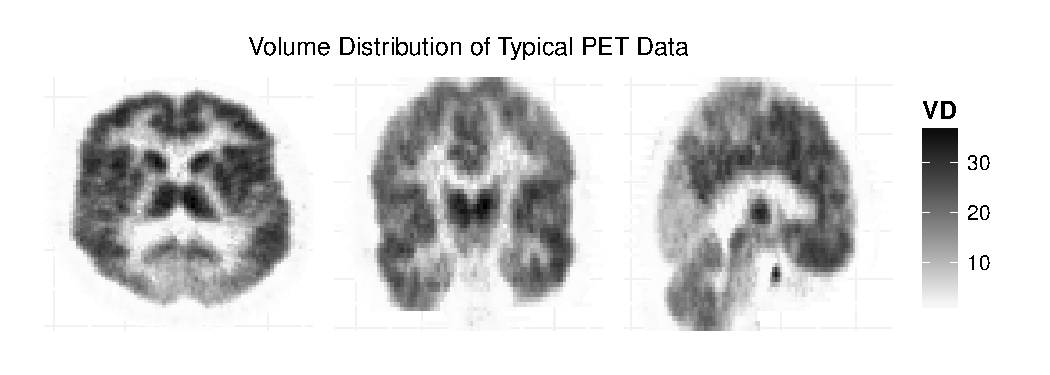
\includegraphics[width=\linewidth]{fig_src/PETPlot-smc2-ps-bw}
  \caption[Volume of distribution of real \protect\pet compartmental model
  data]
  {Estimates of $V_D$ from a single \pet scan as found using \smc[2].
    The data shows that the volume of distribution exhibits substantial
    spatial variation. Note that each pixel in the image represent an estimate
    from an individual time series data set. There are approximately a quarter
    of a million of them and each requires a Monte Carlo simulation to select
    a model.}
  \label{fig:petplot}
\end{figure}


\section{Modeling error structures}
\label{sec:Error models}

In the scenarios considered in this thesis, linear one-, two-, and three-compartment models are considered possible; the methods could deal with other compartmental models straightforwardly, but we focus on these as they are the most interesting in the application of interest. Let $t_1, \dots, t_n$ be the end points of the time frames at which the tissue concentrations are measured, and let $y_1,\dots,y_n$ be the observed data. Measurement error is assumed to be white and additive with zero mean and variance proportional to activities divided by the length of time frames (i.e., $C_T(t_i)/(t_i - t_{i-1})$, the same as the one used in the simulated data). These assumptions arise from the physical characterization of the \pet system of interest; alternative specifications would be possible and appropriate for other situations. Recall Equations~\eqref{eq:CT} and~\eqref{eq:HTP} and rewrite $C_T(t)$ in terms of the parameters $\phi_{1:r}$ and $\theta_{1:r}$, for $i = 1,\dots,n$
\begin{gather*}
  C_T(t_i;\phi_{1:r},\theta_{1:r}) =
  \sum_{j=1}^r \phi_j\int_0^{t_i}C_P(s)e^{-\theta_j(t_j-s)} \intd s \\
  y_i = C_T(t_i;\phi_{1:r},\theta_{1:r}) +
  \varepsilon_i\sqrt{\frac{C_T(t_i;\phi_{1:r},\theta_{1:r})} {t_i - t_{i-1}}},
\end{gather*}
where $r = 1, 2$, or~$3$ is the number of tissue compartments, $t_0 = 0$, and $\varepsilon_i$ are identically independently distributed (i.i.d.) random variables with mean zero. It is usually assumed that $\varepsilon_i$ has a Normal distribution. It is demonstrated in \cite{Zhou2013} that there is evidence that a Student~$t$ distribution better fits the observed data. Therefore, we consider two error structures,
\begin{align*}
  \varepsilon_i &\sim \mathcal{N}(0,\lambda^{-1})
  &\text{Normally-distributed errors} \\
  \varepsilon_i &\sim \mathcal{T}(0,\tau,\nu)
  &\text{$t$-distributed errors},
\end{align*}
where $\mathcal{N}(0,\lambda^{-1})$ is the Normal distribution with mean zero and precision $\lambda$, and $\mathcal{T}(0,\tau,\nu)$ is the Student~$t$ distribution with location zero, scale $\tau$, and degrees of freedom $\nu$. Unless stated otherwise, in the examples of this thesis, the Normally distributed error structure is used when modeling the simulated data. The Student~$t$ distributed error structure is used when modeling the real data.
